\section{Implementation}
\label{implementation}

The first CTFE First was created for the C-=-1 language, using out-of-the-box parser generator and backend.
The most important aspect of implementing a CTFE First compiler is the design of the data structures, described in chapter \ref{data_structures}, that will be used by the interpreter.

Languages that seek to exploit CTFE First approach in design of their compilers, should define a set of data structures to describe user code, i.e. an Semantic Model.
It will allow the programmer to interact and mainpulate the structure of the program at compile-time.
The Semantic model designed and implemented for C-=-1 is described in chapter \ref{semantic_model}.

The final piece of a CTFE First compiler is the Backend Interface.
It is a program, written in the target language, and ran at compile-time that translates the semantic model into the backends assembly language.
Backend Interface implemented for C-=-1 is relativley small and has been described in chapter \ref{implementation/backend-interface}.

\subsection{Interpreter data structures}
\label{data_structures}
Data structures of the C-=-1 Interpreter have been designed ease of development and debugging in mind.
They are thus not particularly efficent.

\begin{figure}
	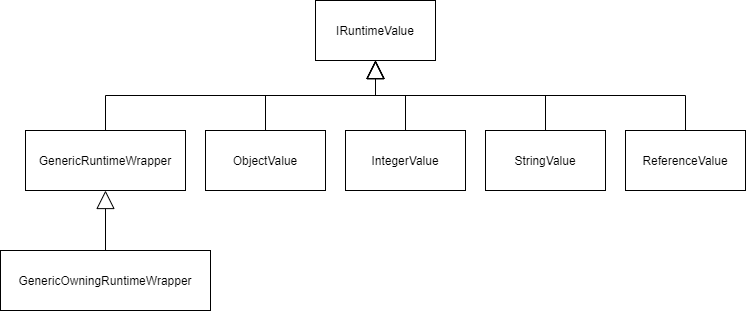
\includegraphics[width=8cm]{pictures/interpreter_data_structures_uml.png}
	\caption{Class diagram of C-=-1 interpreter data structures}
	\label{fig:interpreter_data_structures}
\end{figure}

Figure \ref{fig:interpreter_data_structures} contains a class diagram of most of the types used to represent values within C-=-1.
All of them derive from \lstinline{IRuntimeValue} and are managed via C++ smart pointers.
The interface of the base class allows the value to be converted to a human readable format, serialisation, deserialisation and copying.

The most prymitive types within the hierarchy are \lstinline{StringValue} and \lstinline{IntegerValue}.
They are simple wrappers for strings and integers, present in the host language.
Floating point numbers were not implemented as they were not nessecary for implementation of a basic compiler.

User-defined types are represented using \lstinline{ObjectValue}.
The contents of an objects is kept as a \lstinline{string} - \lstinline{IRuntimeValue} dictionary, with field names as keys and \lstinline{uniqe_ptr<IRuntimeValue>} as values.
C-=-1 object is therefore spread out in memory, even if the fields are directly contained within the class, without any indirection.


There are multiple types of reference within the C-=-1 interpreter.
The most basic pointer type is a reference to C-=-1 value.
It was realised as a pointer to the owning pointer of the value.
The reasoning behind this decision was to allow assigning to the referenced value.

\subsection{Program semantic model}
\label{semantic_model}

A major motivation in creating CTFE First was the ability to support languages with compile-time metaprogramming.
This includes reflection and modification of the code being compiled.
User program had to be represented as a complete and modifiable object, using the interpreters data structures.

C-=-1 language model divides the user program into assemblies.
They represent an individual program package: a library or an executable file.
The compiler is invoked to compile an assembly, together with its dependencies.
Assembly is the root object of C-=-1 program model, it stores a list of assemblies it depends on and the root namespace of the package it represents.
The remainder of user code is organised around namespaces, types, functions and fields.
These parts of the model are repesented by native classes of the host language and form the basis for the rest of the model.

The most complex part of the model is the representation of the function body.
Like in most programming languages, a C-=-1 function can contain a variety of instruction types.
That includes complex statements and blocks of statements that can be arbitrarly nested.
Each instruction may also contain expressions of any complexity.

To deal with this complexity, C-=-1 semantic model for functions is build around two interfaces: \lstinline{IInstruction} and \lstinline{IExpression} and their concrete implementations.

\subsection{Backend interface}
\label{implementation/backend-interface}
